\documentclass[10pt]{exam}
\usepackage[hon]{template-for-exam}
\usepackage{endnotes,graphicx}
\usepackage{tikz,graphicx,enumitem,multicol,float,my-tikz-clipart,silence,cclicenses}
\graphicspath{{./figures/}}
\WarningFilter{latex}{Label `part}
\WarningFilter{latex}{There were multiply-defined labels}

\footer{}{\thepage}{\sc \myclass}


%\def\answer#1{\footnotetext{#1}}
%\def\myquestion{\item\stepcounter{footnote}}

\def\enoteheading{}
\def\answer#1{\endnotetext{#1}}
\def\theanswers{\theendnotes}
\def\myquestion{\item\stepcounter{endnote}}

\newenvironment{myquestions}{
  %\begin{multicols}{2}
  \begin{enumerate}[resume]
}{
  \end{enumerate}
  %\end{multicols}
}
\makeatletter
\patchcmd{\enit@setresumekeys}{\def}{\gdef}{}{}
\patchcmd{\enit@setresumekeys}{\def}{\gdef}{}{}
\makeatother

\newcommand{\myheading}[1]{
  \subsection*{#1}
  \addtoendnotes{\vspace{1em}\par\noindent\textbf{#1}}
}
\newcommand{\mysubheading}[1]{\uplevel{\subsubsubsection*{#1}}
}

\newenvironment{mychoices}[1]{
  \vspace{-1em}
  \begin{multicols}{#1}
  \begin{choices}
}{
  \end{choices}
  \end{multicols}
  \vspace{-1em}
}


\title{Honors Physics - Spring Final Exam Review}
\author{Rohrbach}
\date{\today}

\begin{document}
\maketitle

\section*{Multiple Choice}

\myheading{Ch 8: Momentum}

\subsection*{Vocab}

\begin{multicols}{3}
  \begin{itemize}[itemsep=0pt]
    \item momentum
    \item conservation of momentum
    \item impulse
    \item elastic collision
    \item inelastic collision
  \end{itemize}
\end{multicols}

\subsection*{Questions}


\begin{myquestions}


\myquestion What is conservation of momentum? \answer{A}
\begin{choices}
\choice the total momentum before a collision is equal to the total momentum after a collision
\choice impulse equals change in momentum
\choice two objects stick together after a collision
\choice total momentum of a system is always zero
\end{choices}

\myquestion Why does a gun recoil when a bullet is shot from it? \answer{C}
\begin{choices}
\choice the forward motion of the bullet imparts an impulse on the gun that pushes it backwards
\choice the force of the explosion causes a push on the gun
\choice the forward momentum of the bullet needs to be counteracted by a backward momentum in the gun
\end{choices}

\myquestion Which of the following effects would not decrease the force on an object (such as a dropped egg)? \answer{B}
\begin{choices}
\choice decrease the velocity of the object before the collision
\choice decrease the time of collision
\choice increase the time of collision
\choice decrease the velocity of the object after the collision
\end{choices}

\myquestion After a car accident, the two cars stick together. This is an example of a/an \fillin[][2em] \answer{A} \par
\begin{oneparchoices}
\choice inelastic collision
\choice impulse collision
\choice elastic collision
\choice destructive collision
\end{oneparchoices}

\myquestion How can you use conservation of momentum to explain why a water rocket flies \answer{B}
\begin{choices}
\choice objects on Earth cannot zero momentum, so they must move
\choice if water is forced out the bottom of the rocket, the rocket must launch upwards to conserve momentum
\choice putting water in the rocket gives it an initial momentum in the upward direction
\choice the interaction between the water and the rocket is an inelastic collision, giving it momentum
\end{choices}

\myquestion A bouncy ball and a sphere of putty--each of the same mass--are thrown at a wall with the same inital velocity. The putty sticks to the wall while the ball rebounds back in the direction it came with almost the same velocity. Which of the following is true? \answer{A}
\begin{choices}
\choice The bouncy ball has a greater change in momentum
\choice The putty has a greater change in momentum
\choice The ball and the putty have the same change in momentum
\choice None of these are true.
\end{choices}

\myquestion Consider two unequal masses, $M$ and $m$. Which of the following statements is false? \answer{E}
\begin{choices}
\choice The center of mass is closer to the larger mass.
\choice The center of mass lies on the line joining the centers of each mass.
\choice There is only one center of mass
\choice It is possible for the center of mass to lie within one of the objects.
\choice none of the above
\end{choices}

\myquestion When a cannon fires a cannonball, the cannon will recoil backward because the \answer{B}
\begin{choices}
\choice energy of the cannon is greater than the energy of the cannonball.
\choice momentum of the cannonball and cannon is conserved.
\choice momentum of the cannon is greater than the energy of the cannonball.
\choice energy of the cannonball and cannon is conserved.
\end{choices}

\myquestion A small car meshes with a large truck in a head-on collision. Which of the following statements concerning the magnitude of the average collision force is correct? \answer{A}
\begin{choices}
\choice The small car and the truck experience the same average force.
\choice The small car experiences the greater average force.
\choice The truck experiences the greater average force.
\choice It is impossible to tell since the masses and velocities are not given.
\end{choices}

\myquestion In an inelastic collision, if the momentum is conserved, then which of the following statements is true about kinetic energy? \answer{C}
\begin{mychoices}{2}
\choice Kinetic energy is gained.
\choice Kinetic energy is also conserved.
\choice Kinetic energy is lost.
\choice none of the above
\end{mychoices}

\myquestion A car of mass 2000 kg moves to the right along a level, straight road at a speed of 6.0 m/s. It collides directly with a stopped motorcycle of mass 100 kg. What is the total momentum after the collision? \answer{C}
\begin{choices}
\choice \SI{2000}{kg.m/s} to the right
\choice \SI{6000}{kg.m/s} to the right
\choice \SI{12,000}{kg.m/s} to the right
\choice zero
\choice none of the above
\end{choices}

\myquestion A 2000-kg car traveling at 20 m/s runs into the rear of a stopped car that has a mass of 500 kg and they stick together. What is the speed of the cars after the collision? \answer{C} \par
\begin{oneparchoices}
\choice 10 m/s
\choice 5.0 m/s
\choice 16 m/s
\choice 20 m/s
\choice none of the above
\end{oneparchoices}


\end{myquestions}

\pagebreak

\myheading{Ch 10: Rotation}

\subsection*{Vocab}

\begin{multicols}{3}
  \begin{itemize}[itemsep=0pt]
    \item angular velocity
    \item angular acceleration
    \item torque
    \item radians
    \item angular momentum
    \item moment of inertia
  \end{itemize}
\end{multicols}

\subsection*{Questions}

\begin{myquestions}
  \myquestion An ice skater performs a pirouette (a fast spin) by pulling in his outstretched arms close to his body. What happens to his \textbf{angular momentum} about the axis of rotation? \par \answer{C}
  \begin{oneparchoices}
  \choice it increases.
  \choice it decreases.
  \choice it stays the same
  \choice impossible to say.
  \end{oneparchoices}

  \myquestion An ice skater performs a pirouette (a fast spin) by pulling in his outstretched arms close to his body. What happens to his \textbf{moment of inertia} about the axis of rotation? \par \answer{B}
  \begin{oneparchoices}
  \choice it increases.
  \choice it decreases.
  \choice it stays the same
  \choice impossible to say.
  \end{oneparchoices}

  \myquestion Angular velocity is expressed in units of \answer{A} \par
  \begin{oneparchoices}
  \choice radians per second.
  \choice meters per second.
  \choice arcs per second.
  \choice omegas per second.
  \end{oneparchoices}

  \myquestion Angular acceleration is expressed in units of \answer{D} 
  \begin{mychoices}{2}
  \choice arcs per second squared.
  \choice meters per second squared.
  \choice alphas per second squared.
  \choice radians per second squared.
  \end{mychoices}

  \myquestion Two equal forces are applied to a door. The first force is applied at the midpoint of the door; the second force is applied at the doorknob. Both forces are applied perpendicular to the door. Which force exerts the greater torque? \answer{A}
  \begin{mychoices}{2}
  \choice the second at the doorknob
  \choice the first at the midpoint
  \choice both exert zero torques
  \choice both exert equal non-zero torques
  \end{mychoices}

  \myquestion Two forces are applied to a doorknob, perpendicular to the door. The first force is three times as large as the second force. The ratio of the torque of the first to the torque of the second is \answer{D} \par
  \begin{mychoices}{4}
  \choice 1/4.
  \choice 2.
  \choice 1/3.
  \choice 3.
  \end{mychoices}

  \myquestion If a constant net torque is applied to an object, that object will \answer{D}
  \begin{choices}
  \choice have a decreasing moment of inertia.
  \choice rotate with constant angular displacement.
  \choice rotate with constant angular velocity.
  \choice having an increasing angular velocity.
  \end{choices}

  
  \myquestion Two spheres have the same radius and equal masses. One is made of solid aluminum, and the other is made from a hollow shell of gold. If allowed to race down an inclined plane, which one will reach the bottom first? \answer{A}
  \begin{choices}
  \choice the solid aluminum sphere will reach the bottom first
  \choice the hollow gold sphere will reach the bottom first
  \choice they will reach the bottom at the same time
  \choice it is impossible to tell
  \end{choices}


  \myquestion What is the quantity used to measure an object's resistance to changes in rotation? \answer{B} \par
  \begin{oneparchoices}
  \choice angular velocity ($\omega$)
  \choice moment of inertia ($I$)
  \choice mass ($m$)
  \choice torque ($\tau$)
  \end{oneparchoices}

  \myquestion Little Bobby and Janie are both riding a carousel.  Janie is on a pony, which is 5 m from the center of rotation, and Bobby is on a water buffalo, which is 7 m from the center. The merry-go-round makes one complete revolution every 30 seconds. Which of the following is true? \answer{C} 

  \begin{minipage}[b]{4.2in}
    
    \begin{choices}
      \choice Bobby has larger $v$; Janie has larger $\omega$
      \choice Bobby has larger $\omega$; Janie has larger $v$
      \choice Bobby has larger $v$; both kids have the same $\omega$
      \choice Bobby has larger $\omega$; both kids have the same $v$
      \choice Both kids have the same $\omega$ and the same $v$
    \end{choices}

    \vspace*{4em}
  \end{minipage}
  %
  \begin{minipage}[b]{1.9in}
      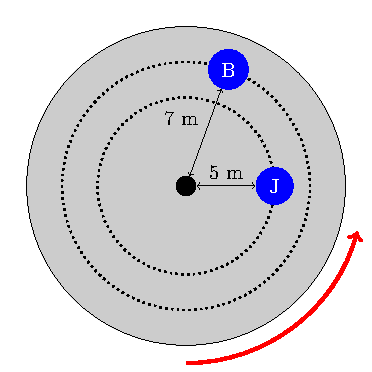
\includegraphics[width=1.9in]{circular.pdf}
  \end{minipage}
  

\end{myquestions}

\myheading{Ch 16: SHM \& Waves}

\subsection*{Vocab}

\begin{multicols}{3}
  \begin{itemize}[itemsep=0pt]
    \item simple harmonic motion
    \item frequency
    \item period
    \item spring constant
    \item amplitude
    \item interference
    \item longitudinal wave
    \item transverse wave
    \item resonance
  \end{itemize}
\end{multicols}


\subsection*{Questions}



\begin{myquestions}


  \myquestion What would happen to the period of a pendulum if you increase the mass? \answer{C} \par
  \begin{oneparchoices}
  \choice period would increase
  \choice period would decrease
  \choice period wouldn't change
  \end{oneparchoices}

  % \myquestion What would happen to the period of a pendulum if you increase the amplitude? \answer{C} \par
  % \begin{oneparchoices}
  % \choice period would increase
  % \choice period would decrease
  % \choice period wouldn't change
  % \end{oneparchoices}

  % \myquestion What would happen to the period of a pendulum if you increase the length? \answer{A} \par
  % \begin{oneparchoices}
  % \choice period would increase
  % \choice period would decrease
  % \choice period wouldn't change
  % \end{oneparchoices}

  % \myquestion What would happen to the period of a pendulum if you increase the acceleration of gravity? \answer{B} \par
  % \begin{oneparchoices}
  % \choice period would increase
  % \choice period would decrease
  % \choice period wouldn't change
  % \end{oneparchoices}

  \myquestion What would happen to the period of a \emph{spring} if you increase the mass? \answer{A} \par
  \begin{oneparchoices}
  \choice period would increase
  \choice period would decrease
  \choice period wouldn't change
  \end{oneparchoices}

  % \myquestion What would happen to the period of a spring if you increase the amplitude? \answer{C} \par
  % \begin{oneparchoices}
  % \choice period would increase
  % \choice period would decrease
  % \choice period wouldn't change
  % \end{oneparchoices}

  % \myquestion What would happen to the period of a spring if you increase the spring constant? \answer{B} \par
  % \begin{oneparchoices}
  % \choice period would increase
  % \choice period would decrease
  % \choice period wouldn't change
  % \end{oneparchoices}

  % \myquestion What would happen to the period of a spring if you increase the acceleration of gravity? \par\answer{C}
  % \begin{oneparchoices}
  % \choice period would increase
  % \choice period would decrease
  % \choice period wouldn't change
  % \end{oneparchoices}

  \myquestion For a spring, what causes the restoring force? \answer{C}
  \begin{mychoices}{2}
  \choice inertia of the mass
  \choice force of gravity
  \choice tension of the spring itself
  \choice there is no restoring force
  \end{mychoices}

  \myquestion Increasing the frequency \fillin[][3em] the period. \answer{B} \par
  \begin{mychoices}{3}
  \choice does not affect
  \choice decreases
  \choice increases
  \end{mychoices}

  \myquestion Why does a pendulum keep moving when it gets to equilibrium? \answer{B}
  \begin{choices}
  \choice the potential energy of the pendulum pulls it up from equilibrium back to the top
  \choice the inertia of the pendulum makes it want to keep moving through equilibrium
  \choice the restoring force pushes it past equilibrium
  \choice the frequency of the pendulum keeps it from stopping
  \end{choices}



  \myquestion A wave in which the particles back-and-forth parallel to the direction of the wave's motion is known as a \fillin[][3em]. \par \answer{B}
  \begin{oneparchoices}
  \choice simple harmonic wave
  \choice longitudinal wave
  \choice transverse wave
  \choice destructive interference
  \end{oneparchoices}

  \uplevel{
  A mass is attached to a spring sitting on a frictionless horizontal surface.  The mass oscillates between the positions $x=-A$ and $x=A$ as shown:

  \begin{center}
    
\includegraphics[width=7cm]{SHM.pdf}
  \end{center}
}
  \myquestion Indicate where the mass will have a velocity of zero. \par \answer{A}
  \begin{mychoices}{4}
    \choice at $x=\pm A$
    \choice at $x=0$
    \choice at $x=\pm A/2$
    \choice never
  \end{mychoices}


  \myquestion Indicate where the mass will have an acceleration of zero. \par \answer{B}
  \begin{mychoices}{4}
    \choice at $x=\pm A$
    \choice at $x=0$
    \choice at $x=\pm A/2$
    \choice never
  \end{mychoices}

  \myquestion What do waves do? \answer{B}
  \begin{choices}
  \choice transport work without transporting power
  \choice transport energy without transporting matter
  \choice move particles from one place to another without transporting energy
  \choice absorb forces while generating energy
  \end{choices}

  \myquestion In a wave, the maximum displacement of points of the wave from equilibrium is called the wave's \par \answer{E}
  \begin{oneparchoices}
  \choice frequency
  \choice speed
  \choice trough
  \choice wavelength
  \choice none of the above
  \end{oneparchoices}

  \myquestion Microwaves have a higher frequency than radio waves. Therefore, which of the following is true? \answer{B}
  \begin{choices}
  \choice microwaves have a longer wavelength than radio waves
  \choice microwaves have a shorter wavelength than radio waves
  \choice microwaves have a faster speed than radio waves
  \choice microwaves have a slower speed than radio waves
  \end{choices}

  \myquestion Two simple pendulums A and B are 3.0 m long. The period of A is $T$. Pendulum A is three times as heavy as pendulum B. What is the period of B? \par \answer{A}
  \begin{mychoices}{4}
  \choice $T$
  \choice $0.71T$
  \choice $2T$
  \choice $1.4T$
  \end{mychoices}

  \myquestion How can sound be used to break glass? \answer{B}
  \begin{choices}
  \choice if sound is played at a sufficiently high frequency the glass will resonate
  \choice if sound is played at a certain frequency the glass will resonate
  \choice if sound is played at a sufficiently high volume the glass will resonate
  \choice if sound is played at a sufficiently high wavelength the glass will resonate
  \end{choices}

  \pagebreak
  \myquestion The distance between successive troughs on a wave is called the wave's \par \answer{C}
  \begin{mychoices}{4}
  \choice frequency
  \choice speed
  \choice wavelength
  \choice amplitude
  \end{mychoices}


  \myquestion Resonance in a system, such as a string fixed at both ends, occurs when \answer{D}
  \begin{choices}
  \choice its frequency is smaller than the frequency of an external source.
  \choice it is oscillating in simple harmonic motion.
  \choice its frequency is greater than the frequency of an external source.
  \choice its frequency is the same as the frequency of an external source.
  \end{choices}

  \myquestion The time for one cycle of a periodic process is called the \par \answer{B}
  \begin{mychoices}{4}
  \choice amplitude.
  \choice period.
  \choice wavelength.
  \choice frequency.
  \end{mychoices}

  \myquestion A 1.0-kg object is attached to a spring of spring constant 10 N/m. The object is displaced by 5.0 cm from the equilibrium position and let go. What is the period of vibration? \par \answer{D}
  \begin{mychoices}{4}
  \choice 8.0 s
  \choice 4.0 s
  \choice 16 s
  \choice 2.0 s
  \end{mychoices}

  \myquestion For a periodic process, the number of cycles per unit time is called the \par \answer{D}
  \begin{mychoices}{4}
  \choice period.
  \choice amplitude.
  \choice wavelength.
  \choice frequency.
  \end{mychoices}

  \myquestion Consider the two waves below. Assume that they are both traveling through the same medium. Which of the following is true? \answer{D}
    %
    \begin{center}
      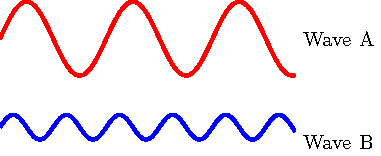
\includegraphics{waves.pdf}
    \end{center}
    %
    \begin{choices}
    \choice Wave B has both a larger wavelength and a higher frequency
    \choice Wave B has a larger wavelength, but Wave A has a higher frequency
    \choice Wave A has both a larger wavelength and a higher frequency
    \choice Wave A has a larger wavelength, but Wave B has a higher frequency
    \end{choices}







\end{myquestions}

\pagebreak
\myheading{Ch 18-21: Electricity}

\subsection*{Vocab}

\begin{multicols}{3}
  \begin{itemize}[itemsep=0pt]
    \item Conductors
    \item Potential difference/Voltage 
    \item Ohm's Law
    \item Electric Field
    \item Ground
    \item Circuits
    \item Current
    \item Resistance
    \item Test charges
  \end{itemize}
\end{multicols}


\subsection*{Questions}
\begin{myquestions}
  \myquestion Two lightbulbs are wired in a series circuit. What happens when one of the bulbs breaks? \answer{B}
  \begin{mychoices}{2}
  \choice the other bulb stays just as bright
  \choice both bulbs go out
  \choice the other bulb gets dimmer
  \choice the other bulb gets brighter
  \end{mychoices}

  \myquestion Two lightbulbs are wired in a parallel circuit. What happens when one of the bulbs breaks? \answer{A}
  \begin{mychoices}{2}
  \choice the other bulb stays just as bright
  \choice both bulbs go out
  \choice the other bulb gets dimmer
  \choice the other bulb gets brighter
  \end{mychoices}

  % \myquestion When you add another resistor to a parallel circuit, \answer{C}
  % \begin{choices}
  % \choice the equivalent resistance stays the same
  % \choice the equivalent resistance goes up
  % \choice the equivalent resistance goes down
  % \choice the equivalent resistance goes to zero
  % \end{choices}

  \myquestion Which of the statements is true? \answer{B}
  \begin{choices}
  \choice resistance and current are directly proportional
  \choice voltage and current are directly proportional
  \choice resistance and charge are directly proportional
  \choice two of the above are true
  \end{choices}

  \myquestion Which of the following is NOT true for a series circuit? \answer{A}
  \begin{choices}
  \choice The voltage across each resistor is the same as the battery's voltage
  \choice The current through each resistor is the same as the current out of the battery
  \choice The sum of the voltages across each resistor is the same as the battery's voltage
  \choice The equivalent resistance is larger than the resistance of any individual resistor
  \end{choices}

  \myquestion Which of the following is NOT true for a parallel circuit? \answer{B}
  \begin{choices}
  \choice The voltage across each resistor is the same as the batterys voltage
  \choice The current through each resistor is the same as the current out of the battery
  \choice The sum of the current through each resistor is the same as the current out of the battery
  \choice The equivalent resistance is smaller than the resistance of any individual resistor
  \end{choices}

  \myquestion An ampere is a unit of electrical \par \answer{E}
  \begin{oneparchoices}
  \choice voltage
  \choice resistance
  \choice pressure
  \choice all of these
  \choice none of these
  \end{oneparchoices}

  \myquestion Two protons attract each other gravitationally and repel each other electrically. By far the smaller is \par \answer{B}
  \begin{oneparchoices}
  \choice the electrical repulsion.
  \choice the gravitational attraction.
  \choice neither - they are the same.
  \end{oneparchoices}

  \myquestion Two charged particles attract each other with a force $F$. If the charges of both particles are tripled, and the distance between them tripled, then the force of attraction will be \par \answer{C}
  \begin{oneparchoices}
  \choice $F/4$.
  \choice $F/2$.
  \choice $F$.
  \choice $2F$.
  \choice none of these.
  \end{oneparchoices}

  \myquestion Two charged particles repel each other with a force $F$. If the charge of one of the particles is doubled and the distance between them is doubled, then the force will be \par \answer{A}
  \begin{oneparchoices}
  \choice $F/2$.
  \choice $2F$.
  \choice $F/4$.
  \choice $F$.
  \choice none of these.
  \end{oneparchoices}

  \myquestion Two charged objects are separated by a distance $d$. The first charge is larger in magnitude than the second charge. \answer{D}
  \begin{choices}
  \choice The charges exert forces on each other equal in magnitude and pointing in the same direction.
  \choice The second charge exerts a larger force on the first charge.
  \choice The first charge exerts a larger force on the second charge.
  \choice The charges exert forces on each other equal in magnitude and opposite in direction.
  \end{choices}

  \myquestion Two charges separated by one meter exert 1-N forces on each other. If the charges are pushed to 1/2 meter separation, the force on each charge will be \par \answer{C}
  \begin{mychoices}{5}
  \choice 1 N.
  \choice 2 N.
  \choice 4 N.
  \choice 8 N.
  \choice 16 N.
  \end{mychoices}

  % \myquestion Two charges separated by one meter exert 1-N forces on each other. If the charges are pulled to 2-m separation distance, the force on each charge will be \par \answer{A}
  % \begin{oneparchoices}
  % \choice 0.25 N.
  % \choice 0.11 N.
  % \choice 0 N.
  % \choice 4 N.
  % \choice none of the above.
  % \end{oneparchoices}

  \myquestion The total amount of charge that passes through a wire's full cross section at any point per unit of time is referred to as a \par \answer{B}
  \begin{oneparchoices}
  \choice voltage.
  \choice current.
  \choice wattage.
  \choice electric potential.
  \end{oneparchoices}

  \myquestion Consider the circuit below. Which of the following is true? \answer{A}

     \begin{center}
       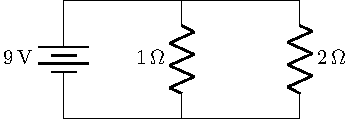
\includegraphics{circuit.pdf}
     \end{center}

    \begin{choices}
      \choice the 1-ohm resistors has more current flowing through it than the 2-ohm resistor
      \choice the 2-ohm resistors has more current flowing through it than the 1-ohm resistor
      \choice there is a larger potential difference accross the 1-ohm resistor than the 2-ohm resistor
      \choice there is a larger potential difference accross the 2-ohm resistor than the 1-ohm resistor
      \choice Both (a) \& (c)
      \choice Both (b) \& (d)
    \end{choices}
    





  \myquestion What happens to the current through the battery when more resistors are added in series. \par \answer{B}
  \begin{oneparchoices}
  \choice current increases
  \choice current decreases
  \choice current stays the same
  \choice impossible to say
  \end{oneparchoices}

  \myquestion What happens to the current through the battery when more resistors are added in parallel? \par \answer{A}
  \begin{oneparchoices}
  \choice current increases
  \choice current decreases
  \choice current stays the same
  \choice impossible to say
  \end{oneparchoices}

\myquestion A main difference between gravitational and electric forces is that electrical forces  \answer{E}
  \begin{choices}
  \choice attract.
  \choice are weaker.
  \choice act over shorter distances.
  \choice obey the inverse-square law.
  \choice are much stronger.
  \end{choices}

  
\end{myquestions}

\pagebreak

\myheading{Ch 25: Geometric Optics}

\subsection*{Vocab}

\begin{multicols}{3}
  \begin{itemize}[itemsep=0pt]
    \item refraction
    \item reflection
    \item real image 
    \item virtual image
    \item focal length
  \end{itemize}
\end{multicols}


\subsection*{Questions}

\begin{myquestions}
  \myquestion The law of reflection states: \answer{D}
  \begin{choices}
  \choice incoming light reflects along the same path that it came
  \choice light bends when it goes from one medium to another
  \choice you can only see your reflection on smooth surfaces
  \choice the angle of incidence is equal to the angle of reflection
  \end{choices}

  \myquestion What is refraction? \answer{A}
  \begin{choices}
  \choice when light bends because it changes speed
  \choice when light bends because it changes frequency
  \choice when light changes color after going through a prism
  \choice when light bounces back through the medium it came from
  \end{choices}

  \myquestion How does a lens work? \answer{D}
  \begin{choices}
  \choice the lens disperses light toward the focal point
  \choice the lens interferes light toward a focal point
  \choice the lens reflects light toward a focal point
  \choice the lens refracts light toward a focal point
  \end{choices}

  \myquestion The angle of reflection \answer{D}
  \begin{choices}
  \choice is always less than the angle of incidence.
  \choice is always greater than the angle of incidence.
  \choice may be greater than or less than the angle of incidence.
  \choice none of the above
  \end{choices}

  \myquestion The principle on which mirrors work is \par \answer{D}
  \begin{mychoices}{4}
  \choice polarization.
  \choice dispersion.
  \choice refraction.
  \choice reflection.
  \end{mychoices}

  \myquestion Light arriving at a concave mirror on a path through the center is reflected \answer{B}
  \begin{mychoices}{2}
  \choice through the focal point.
  \choice back on itself.
  \choice back parallel to the axis.
  \choice through the vertex of the mirror.
  \end{mychoices}

  \myquestion Which of the following is true about light when it enters a new medium that causes its speed to slow down. \answer{B}
  \begin{choices}
  \choice the wavelength of the light increases
  \choice the wavelength of the light decreases
  \choice the frequency of the light increases
  \choice the frequency of the light increases
  \end{choices}

  \pagebreak
  \myquestion In a converging lens, where must the object be in order for the image to be real? \answer{B}
  \begin{choices}
  \choice inside the focal point
  \choice outside the focal point
  \choice at the focal point
  \choice converging lenses never make real images
  \end{choices}

  \myquestion A spherical mirror on which reflection takes place on the inner surface of the sphere is referred to as a \par \answer{B}
  \begin{mychoices}{2}
  \choice convex mirror.
  \choice concave mirror.
  \end{mychoices}

  \myquestion A spherical mirror on which reflection takes place on the outer surface of the sphere is referred to as a \par \answer{A}
  \begin{mychoices}{2}
  \choice convex mirror.
  \choice concave mirror.
  \end{mychoices}

  
\end{myquestions}

\pagebreak

\section*{Problems}
\addtoendnotes{\vspace{1em}\par\noindent\textbf{Problems}}




  \begin{multicols}{2}
    \begin{myquestions}
    \myquestion A 1550-kg car moving south at 10 m/s collides with at 2550-kg car moving north. The cars stick together and move as a unit after the collision with a velocity of 5.22 m/s to the north. Find the velocity of the 2550-kg car before the collision. \answer{14.47 m/s}


    \myquestion James Bond is sitting in the middle of a frictionless pond and left to die by an evil villain who knows nothing about physics. Bond, who is at rest and has a mass of 75.2 kg (including his shoes) takes one of his shoes (m = 2.2 kg) and throws it in the opposite direction he wants to move with a velocity of 20 m/s. With what velocity will Bond move? \answer{0.603 m/s}

    \myquestion The spring in a grocery produce scale is stretched 0.03 meters when 2 kg of oranges are placed in the basket. (a) What is the spring constant? (b) If allowed to oscillate, what will the period of oscillation be? \answer{(a) 653.3 N/m; (b) 0.348 s}

    \myquestion A pendulum makes 9 oscillations in 15 seconds. Find the period and frequency of the pendulum. \answer{T = 1.67 s; f = 0.6 Hz}

    \end{myquestions}
  \end{multicols}
  

  \pagebreak

  \begin{multicols}{2}
    \begin{myquestions}

      \myquestion Red light has a wavelength of \SI{5.90e-7}{m}. What is the frequency of red light?   The speed of light is \SI{3.00e8}{m/s}. \answer{\SI{5.08e14}{Hz}} 

      % \myquestion The pendulum on a grandfather clock swings back and forth 30 times in one minute. What is the length of this pendulum? \answer{0.99 m}

      \myquestion A charge $Q$ of $+7.7 \times 10^{-5}$ C sits at the origin. (a) What is the electric field at $x = +0.64$ meters? (b) If a charge of $-1.8 \times 10^{-6}$ C is placed at that location, what force will it experience? (make sure to include directions!) \answer{(a) \SI{1.69e6}{N/C} (+); \\ \hfill (b) \SI{3.05}{N} (-)}


      \myquestion Three charges ($q_1 = 4.1 \times 10^{-5}$ C, $q_2 = 6.6 \times 10^{-5}$ C, and $q_3 = -1.3 \times 10^{-5}$ C) are situated 0.1 meters from each other. What is the force acting on $q_2$? \answer{3207.6 N}
      %
      \begin{center}
        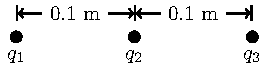
\includegraphics{MultiCharge.pdf}
      \end{center}

    \end{myquestions}

    
  \end{multicols}
  
  \pagebreak
  \begin{multicols}{2}
    \begin{myquestions}
       \myquestion A 200-ohm resistor is connected across 220 V. What current will flow? \answer{1.1 A}

      \myquestion What potential difference is required to cause 4.00 A to flow through a resistance of 120 ohms? \answer{480 V}

      \myquestion Consider a \textbf{diverging} lens with a focal length of 3 cm. An object is 4 cm away. (a) What is the distance between the lens and the image? (b) What is the magnification of the image? (c) Is the image real or virtual? How do you know? \answer{(a) -1.71 cm; (b) 0.43; (c) virtual because $d_i<0$}

      \myquestion A beam strikes a pane of glass at an angle of 32 degrees from the normal. If the index of refraction of the glass is 1.56, and the index of refraction of air is approximately 1.00, what is the angle of refraction? \answer{$19.9^\circ$}
    \end{myquestions}
    
  \end{multicols}




\pagebreak

\section*{Answers}

  \renewcommand{\enotesize}{\normalsize}
  \renewcommand{\enoteformat}{%
    \leftskip=1.8em
    \makebox[0pt][r]{\theenmark. }%
  }

  \hfill

  \begin{multicols}{3}
    \theanswers
  \end{multicols}

\end{document}